
%(BEGIN_QUESTION)
% Copyright 2005, Tony R. Kuphaldt, released under the Creative Commons Attribution License (v 1.0)
% This means you may do almost anything with this work of mine, so long as you give me proper credit

Choose the right type of bipolar junction transistor for each of these switching applications, drawing the correct transistor symbol inside each circle:

$$\includegraphics[width=15.5cm]{i01007x01.eps}$$

\underbar{file i01007}
%(END_QUESTION)





%(BEGIN_ANSWER)

$$\includegraphics[width=15.5cm]{i01007x02.eps}$$

\vskip 10pt

Follow-up question: explain why neither of the following transistor circuits will work.  When the pushbutton switch is actuated, the load remains de-energized:

$$\includegraphics[width=15.5cm]{i01007x03.eps}$$

%(END_ANSWER)





%(BEGIN_NOTES)


%INDEX% Transistor switch circuits: sourcing versus sinking 
%INDEX% Electronics review, transistor switch circuit (BJT)

%(END_NOTES)


